%! TEX root = ../cs251.tex

\textit{Data structures} are collections of data values, the relationships among them, and the functions or operations that can be applied to the data. All three characteristics need to be present.

\section{Array}

\textit{Array} is a linear container of items.

\begin{center}
  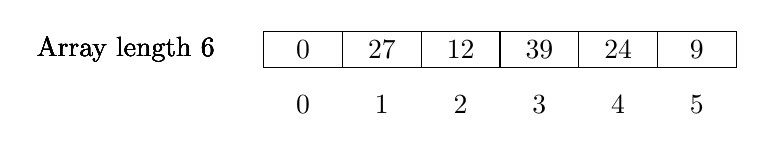
\begin{tikzpicture}
    \foreach \x [ evaluate={\l=int(mod(\x * 69, 42)}; ] in {0,...,5} {
      \node [left] at (-1,1) {Array length 6};
      \node [draw, minimum width=1cm] at (\x, 1) {$\l$};
      \node at (\x, 0.3) {\x};
    } % foreach
  \end{tikzpicture}
\end{center}

\begin{itemize}
  \item Access time: $\Theta (1)$
  \item Inserting $n$ items in the \textit{tail} for array size $n$: $\Theta(1)$ per item, $n \times \Theta(1) \in \Theta(1)$
  \item Inserting $n$ items in the \textit{tail} for array size \textit{unknown}: $\Theta(n)$ per item, $n \times \Theta(n) \in \Theta(n)$
  \item Resizing: $\Theta (n)$
\end{itemize}

Lesson? \textbf{Keep track of the size!}

\section{Linked List}

% https://tex.stackexchange.com/a/19288
\begin{center}
   \begin{tikzpicture} [list/.style={rectangle split, rectangle split parts=2, draw, rectangle split horizontal}, >=stealth, start chain]
     \node[list,on chain] (A) {12};
     \node[list,on chain] (B) {99};
     \node[list,on chain] (C) {37};
     \node[on chain,draw,inner sep=6pt] (D) {};
     \draw (D.north east) -- (D.south west);
     \draw (D.north west) -- (D.south east);
     \draw[*->] let \p1 = (A.two), \p2 = (A.center) in (\x1,\y2) -- (B);
     \draw[*->] let \p1 = (B.two), \p2 = (B.center) in (\x1,\y2) -- (C);
     \draw[*->] let \p1 = (C.two), \p2 = (C.center) in (\x1,\y2) -- (D);
   \end{tikzpicture}
\end{center}

\begin{itemize}
  \item Access time: $\Theta (n)$
  \item Insertion: $\Theta(1)$
  \item Deletion:
    \begin{itemize}
      \item Singly LL: $O(n)$
      \item Doubly LL: $\Theta (1)$
    \end{itemize}
\end{itemize}

\section{Stack}

\begin{verbatim}
-         -        -        7       -      -      -
-         -        5        5       5      -      -     Error
-         3        3        3       3      3      -
init()  push(3)  push(5)  push(7)  pop()  pop()  pop()  pop()
\end{verbatim}

\noindent Stack is a "last in, first out" (LIFO) data structure.

\begin{itemize}
  \item \texttt{push(item)}: Inserting an item on the top -- $\Theta (1)$
  \item \texttt{pop()}: Removes and returns the item on the top -- $\Theta (1)$
  \item \texttt{peek()}: Returns the item on the top
  \item \texttt{size()}: Returns the number of item in the stack
  \item \texttt{isEmpty()}: Checks if size == 0
\end{itemize}

\section{Queue}

\begin{verbatim}
- - -    3 - -   3 5 -   3 5 7   - 5 7   - - 7   - - -   Error
init()   e(3)    e(5)    e(7)     d()     d()     d()     d()
\end{verbatim}

\noindent Queue is a "first in, first out" (FIFO) data structure.

\begin{itemize}
  \item \texttt{enqueue(item)}: Inserts an item at the end - **Theta(1)**
  \item \texttt{dequeue()}: Removes the item at the front of the queue and return it - **Theta(1)**
  \item \texttt{peek()}: Returns the item at the front of the queue w/o removing it
  \item \texttt{size()}: Returns the number of the items in the queue
  \item \texttt{isEmpty()}: Checks if size == 0
\end{itemize}

\subsection{Implementing Queue Using a Circular Array}

\noindent \hrulefill
\begin{algorithmic}[1]
  \Function{Constructor}{$k$} \Comment{$k$ is the initial size of the array}
  \State $Q \gets$ an array of size $k$
  \State size $\gets 0$
  \State head $\gets 0$
  \State tail $\gets k - 1$
  \EndFunction
\end{algorithmic}

\begin{algorithmic}[1]
  \Function{enQueue}{$n$} \Comment{$n$ is the new item to add}
  \If{size $= k$}
    \Return False
  \EndIf
  \item[]
  \State tail $\gets$ (tail + 1) $\mod k$
  \State Q[tail] $\gets n$
  \State size $\gets$ size $+ 1$
  \EndFunction
\end{algorithmic}

\begin{algorithmic}[1]
  \Function{deQueue}{}
  \If{size $= 0$}
    \Return False
  \EndIf
  \item[]
  \State tmp $\gets$ Q[head]
  \State Q[head] $\gets$ nil
  \State head $\gets$ (head + 1) $\mod k$
  \State size $\gets$ size $- 1$
  \item[]
  \Return tmp
  \EndFunction
\end{algorithmic}
\noindent \hrulefill

\section{Tree}

\begin{itemize}
  \item Search: $O(\log(n))$ for a balanced tree (right), $O(n)$ for unbalanced tree (left)
    \begin{multicols}{2}
      \begin{forest}
        for tree={ very thin, circle, draw },
        [{ $8$ } % lv 0
        %
        [{ $4$ }
        %
        [{ $2$ }
        [{ $1$ }]
        [{ $3$ }]
        ]
        %
        [{ $6$ }
        [{ $7$ }]
        ]
        ]
        %
        [{ $12$ }
        %
        [{ $10$ }
        [{ $9$ }]
        [{ $11$ }]
        ]
        %
        [{ $12$ }
        ]
        ]
        ]
      \end{forest}

      \begin{forest}
        for tree={ very thin, circle, draw },
        [{ $5$ } % lv 0
        [{ $4$ }
        [{ $3$ }
        [{ $2$ }
        [{ $1$ }
        ]
        ]
        ]
        ]
        [{}]
        ]
      \end{forest}
    \end{multicols}
  \item \textbf{Maximum number of leaves:} $2^{h}$, where $h$ is the height of the tree
  \item \textbf{Maximum number of nodes:} $\sum^{h}_{i=0} 2^i = 2^{h + 1} - 1$, where $h$ is the height of the tree
\end{itemize}

Following calculations and traversals will be explained using the following \textbf {full binary tree}.

\begin{center}
  \begin{forest}
    for tree={ very thin, circle, draw },
    [{ A } % lv 0
    %
    [{ B }
    %
    [{ D }]
    %
    [{ E }]
    ]
    %
    [{ C }
    %
    [{ F }]
    [{ G }]
    %
    ]
    ]
  \end{forest}
\end{center}

Definitions:

\begin{itemize}
  \item $I$ (number of internal nodes) $= 3$ (A, B, C -- root is an internal node unless it is a leaf)
  \item $N$ (number of nodes) $= 7$
  \item $L$ (number of leaves) $= 4$
\end{itemize}

Full binary tree properties:

\begin{itemize}
  \item $L = I + 1 = \frac{N + 1}{2}$
  \item $N = 2I + 1 = 2L - 1$
  \item $I = \frac{N - 1}{2} = L - 1$
\end{itemize}

Traversal (applicable for all trees, including non-full-binary trees):

\begin{itemize}
  \item \textbf{Preorder -- [N]ode [L]eft [R]ight:} A B D E C F G
  \item \textbf{Inorder -- [L][N][R]:} D B E A F C
  \item \textbf{Postorder -- [L][R][N]:} D E B F C A
  \item Level -- by height: A B C D E F
\end{itemize}

\section{Binary Heap}

\begin{itemize}
  \item Max heap: Key in each node is larger than or equal to the keys in node's two children
  \item Min heap: Key in each node is less than or equal to the keys in node's two children
\end{itemize}

Array implementation for the above max-heap is as follow:

\begin{itemize}
  \item \textproc{Left-child($i$)} = $2i + 1$
  \item \textproc{Right-child($i$)} = $2i + 2$
  \item \textproc{Parent($i$)} = $\lfloor \frac{i - 1}{2} \rfloor$, $i > 0$
\end{itemize}

\subsection{Heapify}

\begin{enumerate}
  \item Define a function \textproc{max-heapify} that given an index $i$, it "sinks down" $A[i]$ to find its correct heap position.
  \item Starting at the last non-leaf node (i.e., parent of the last node), run \textproc{max-heapify} to heapify the subtree.
  
\end{enumerate}
$O(n)$

\begin{python}
def max_heapify(arr, i):
    n = len(arr)

    l = 2 * i + 1
    r = 2 * i + 2

    largest = i
    if l < n and arr[l] > arr[i]:
        largest = l

    if r < n and arr[r] > arr[largest]:
        largest = r

    if largest != i:
        arr[i], arr[largest] = arr[largest], arr[i]
        max_heapify(arr, largest)


def build_heap(arr):
    n = len(arr)

    lastLeftNode = (n // 2) - 1  # floor(n / 2) - 1
    for i in range(lastLeftNode, -1, -1):
        max_heapify(arr, i)
\end{python}

\noindent

